\documentclass{article}

\usepackage{fancyhdr}
\usepackage{extramarks}
\usepackage{amsmath}
\usepackage{amsthm}
\usepackage{amsfonts}
\usepackage{tikz}
\usepackage[plain]{algorithm}
\usepackage{algpseudocode}
\usepackage{enumerate}
\usepackage{tikz}
\usepackage{pythonhighlight}
\usetikzlibrary{automata,positioning}

%
% Basic Document Settings
%  

\topmargin=-0.45in
\evensidemargin=0in
\oddsidemargin=0in
\textwidth=6.5in
\textheight=9.0in
\headsep=0.25in

\linespread{1.1}

\pagestyle{fancy}
\lhead{\hmwkAuthorName}
\chead{\hmwkClass : \hmwkTitle}
\rhead{\firstxmark}
\lfoot{\lastxmark}
\cfoot{\thepage}

\renewcommand\headrulewidth{0.4pt}
\renewcommand\footrulewidth{0.4pt}

\setlength\parindent{0pt}

%
% Create Problem Sections
%

\newcommand{\enterProblemHeader}[1]{
    \nobreak\extramarks{}{Problem \arabic{#1} continued on next page\ldots}\nobreak{}
    \nobreak\extramarks{Problem \arabic{#1} (continued)}{Problem \arabic{#1} continued on next page\ldots}\nobreak{}
}

\newcommand{\exitProblemHeader}[1]{
    \nobreak\extramarks{Problem \arabic{#1} (continued)}{Problem \arabic{#1} continued on next page\ldots}\nobreak{}
    \stepcounter{#1}
    \nobreak\extramarks{Problem \arabic{#1}}{}\nobreak{}
}

\newcommand*\circled[1]{\tikz[baseline=(char.base)]{
		\node[shape=circle,draw,inner sep=2pt] (char) {#1};}}


\setcounter{secnumdepth}{0}
\newcounter{partCounter}
\newcounter{homeworkProblemCounter}
\setcounter{homeworkProblemCounter}{1}
\nobreak\extramarks{Problem \arabic{homeworkProblemCounter}}{}\nobreak{}

%
% Homework Problem Environment
%
% This environment takes an optional argument. When given, it will adjust the
% problem counter. This is useful for when the problems given for your
% assignment aren't sequential. See the last 3 problems of this template for an
% example.
%

\newenvironment{homeworkProblem}[1][-1]{
    \ifnum#1>0
        \setcounter{homeworkProblemCounter}{#1}
    \fi
    \section{Problem \arabic{homeworkProblemCounter}}
    \setcounter{partCounter}{1}
    \enterProblemHeader{homeworkProblemCounter}
}{
    \exitProblemHeader{homeworkProblemCounter}
}

%
% Homework Details
%   - Title
%   - Class
%   - Due date
%   - Name
%   - Student ID

\newcommand{\hmwkTitle}{Homework\ \#10}
\newcommand{\hmwkClass}{Probability \& Statistics for EECS}
\newcommand{\hmwkDueDate}{May 19, 2024}
\newcommand{\hmwkAuthorName}{Fei Pang}
\newcommand{\hmwkAuthorID}{2022533153}


%
% Title Page
%

\title{
    \vspace{2in}
    \textmd{\textbf{\hmwkClass:\\  \hmwkTitle}}\\
    \normalsize\vspace{0.1in}\small{Due\ on\ \hmwkDueDate\ at 23:59}\\
	\vspace{4in}
}

\author{
	Name: \textbf{\hmwkAuthorName} \\
	Student ID: \hmwkAuthorID}
\date{}

\renewcommand{\part}[1]{\textbf{\large Part \Alph{partCounter}}\stepcounter{partCounter}\\}

%
% Various Helper Commands
%

% Useful for algorithms
\newcommand{\alg}[1]{\textsc{\bfseries \footnotesize #1}}
% For derivatives
\newcommand{\deriv}[1]{\frac{\mathrm{d}}{\mathrm{d}x} (#1)}
% For partial derivatives
\newcommand{\pderiv}[2]{\frac{\partial}{\partial #1} (#2)}
% Integral dx
\newcommand{\dx}{\mathrm{d}x}
% Alias for the Solution section header
\newcommand{\solution}{\textbf{\large Solution}}
% Probability commands: Expectation, Variance, Covariance, Bias
\newcommand{\E}{\mathrm{E}}
\newcommand{\Var}{\mathrm{Var}}
\newcommand{\Cov}{\mathrm{Cov}}
\newcommand{\Bias}{\mathrm{Bias}}

\begin{document}

\maketitle

\pagebreak

\begin{homeworkProblem}[1]
    We use python to simulate the result. The code is below:

\begin{python}
    import numpy as np

    # Function to calculate N for a given sample of U values
    def calculate_N(U):
        product = 1
        for i, u in enumerate(U, 1):
            product *= u
            if product < np.exp(-1):
                return i - 1  # Return the index of the last element where the product was less than e^-1
        return len(U)  # If the product never goes below e^-1, return the total count of U values

    # Generate 5000 samples of N
    sample_size = 5000
    Ns = []

    for _ in range(sample_size):
        U = np.random.uniform(0, 1, 1000)  # Generate 1000 uniform random variables
        N = calculate_N(U)
        Ns.append(N)

    # (a) Estimate E(N) using sample mean
    mean_N = np.mean(Ns)
    print("Estimated E(N):", mean_N)

    # (b) Estimate Var(N) using sample variance
    var_N = np.var(Ns)
    print("Estimated Var(N):", var_N)

    # (c) Estimate P(N = i) for i = 0, 1, 2, 3
    counts = np.bincount(Ns)
    probabilities = counts / sample_size
    for i, prob in enumerate(probabilities):
        print("Estimated P(N = {}): {:.4f}".format(i, prob))
\end{python}

Estimated $E(N)$: 0.9896\\
Estimated $Var(N)$: 1.0118918399999999\\
Estimated $P(N = 0)$: 0.3754\\
Estimated $P(N = 1)$: 0.3654\\
Estimated $P(N = 2)$: 0.1780\\
Estimated $P(N = 3)$: 0.0610
\end{homeworkProblem}


\begin{homeworkProblem}[2]
    We use python to simulate the result. The code is below:
\begin{python}
import numpy as np
import matplotlib.pyplot as plt

def plot_bivariate_normal(rho):
    # Define parameters
    mean = [0, 0]
    cov = [[1, rho], [rho, 1]]  # covariance matrix

    # Generate samples from standard normal distribution
    z = np.random.normal(0, 1, 1000)
    w = np.random.normal(0, 1, 1000)

    # Transform samples to bivariate normal distribution
    x = z
    y = rho * z + np.sqrt(1 - rho**2) * w

    # Plot joint PDF
    plt.figure(figsize=(8, 6))
    plt.hist2d(x, y, bins=30, density=True, cmap='Blues')
    plt.colorbar(label='Probability Density')
    plt.xlabel('X')
    plt.ylabel('Y')
    plt.title('Joint PDF of Bivariate Normal Distribution with ρ = {}'.format(rho))

    # Plot isocontour
    x_range = np.linspace(-3, 3, 100)
    y_range = np.linspace(-3, 3, 100)
    X, Y = np.meshgrid(x_range, y_range)
    Z = np.exp(-(X**2 + Y**2 - 2 * rho * X * Y) / (2 * (1 - rho**2))) / (2 * np.pi * np.sqrt(1 - rho**2))
    plt.contour(X, Y, Z, colors='red', linewidths=1)
    plt.show()

# Generate and plot for each rho value
rhos = [0.1, 0.4, 0.7, 0.9]
for rho in rhos:
    plot_bivariate_normal(rho)

\end{python}

\begin{figure}[htbp]
    \centering
    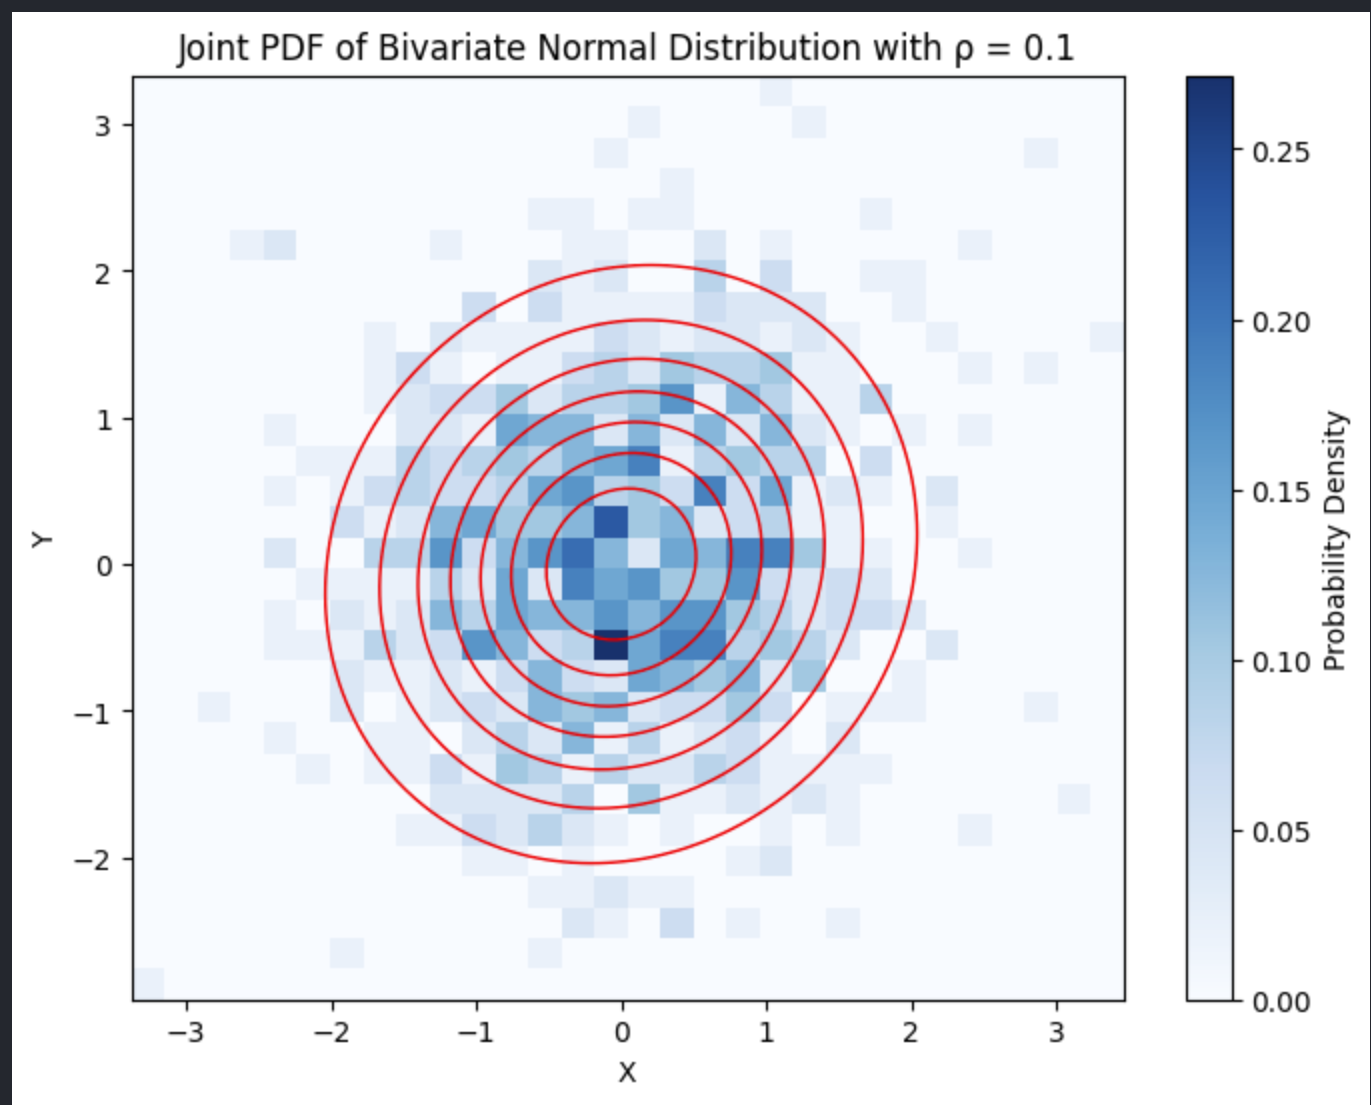
\includegraphics[width=0.23\textwidth]{0.1.png}\hfill
    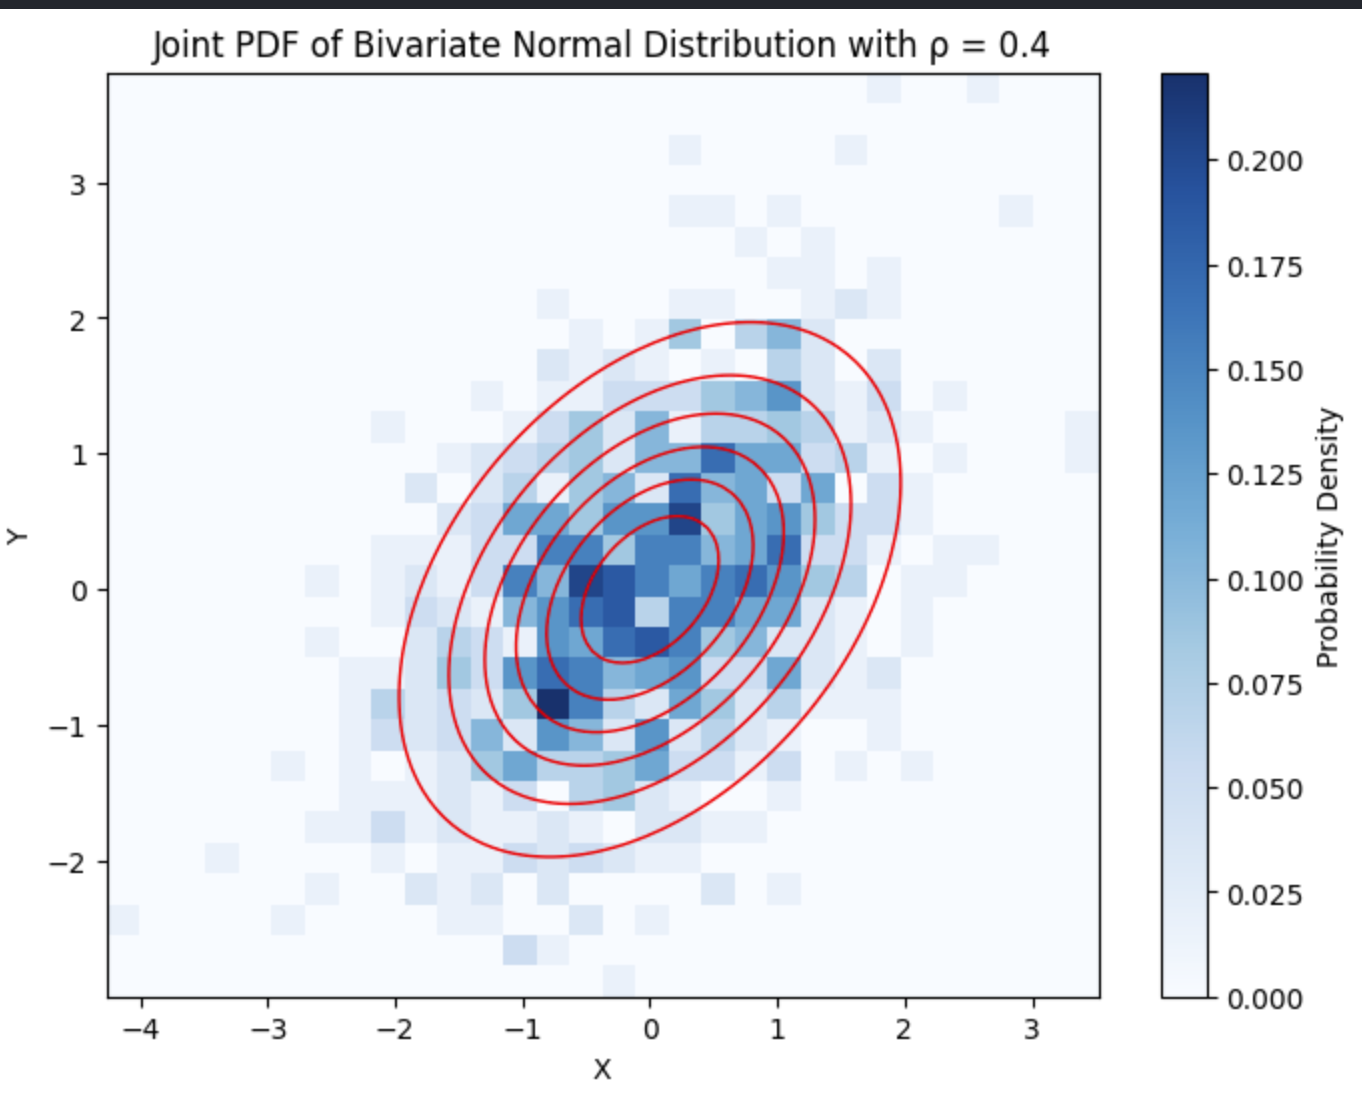
\includegraphics[width=0.23\textwidth]{0.3.png}\hfill
    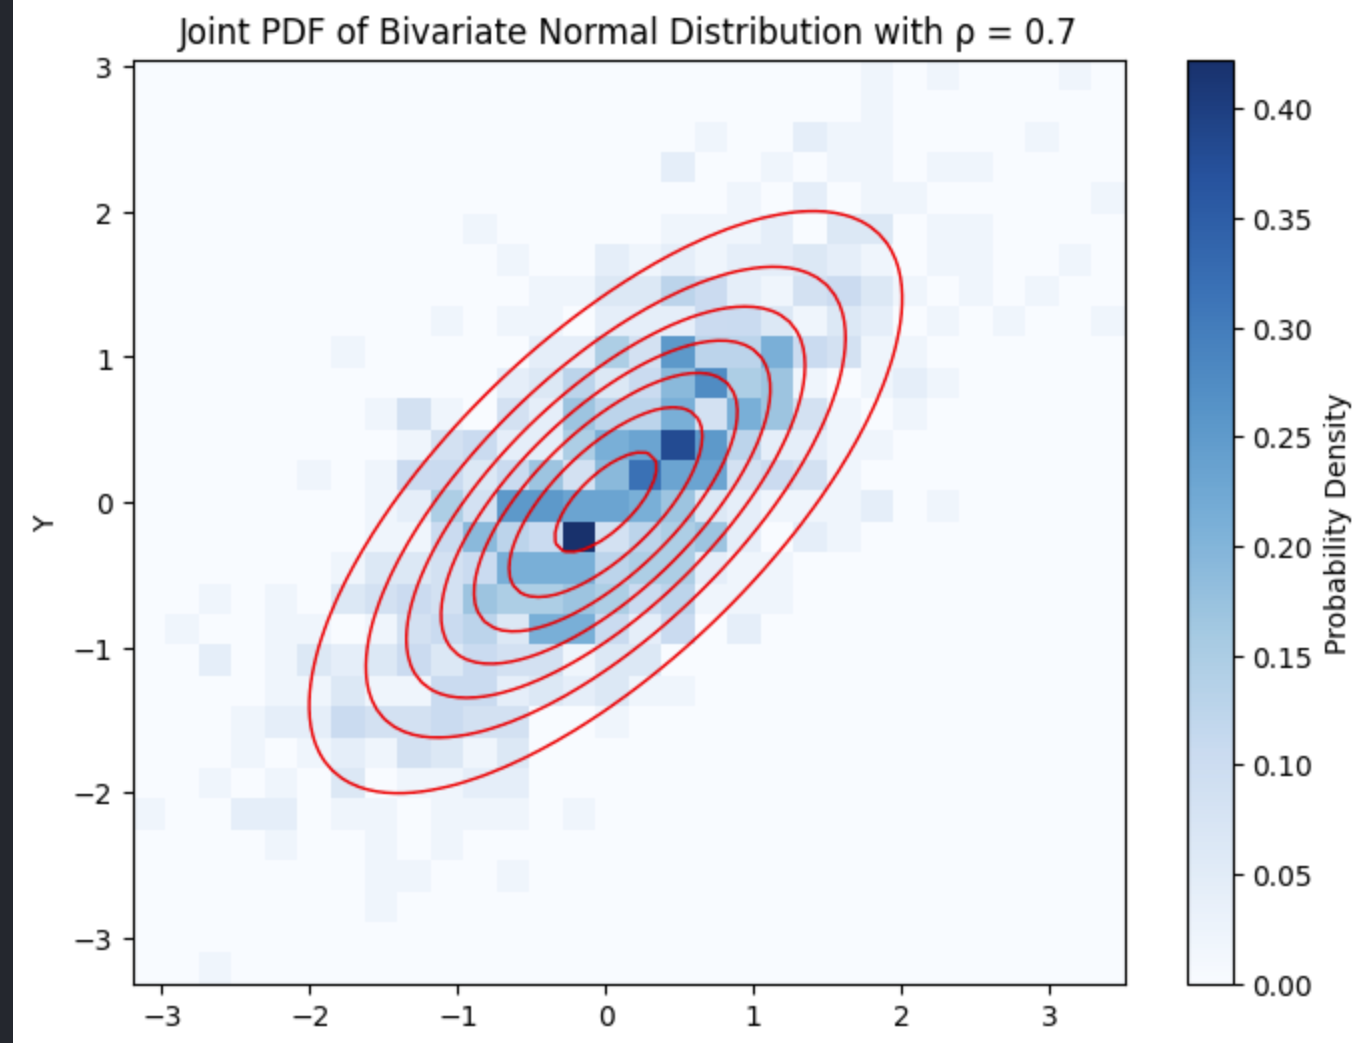
\includegraphics[width=0.23\textwidth]{0.7.png}\hfill
    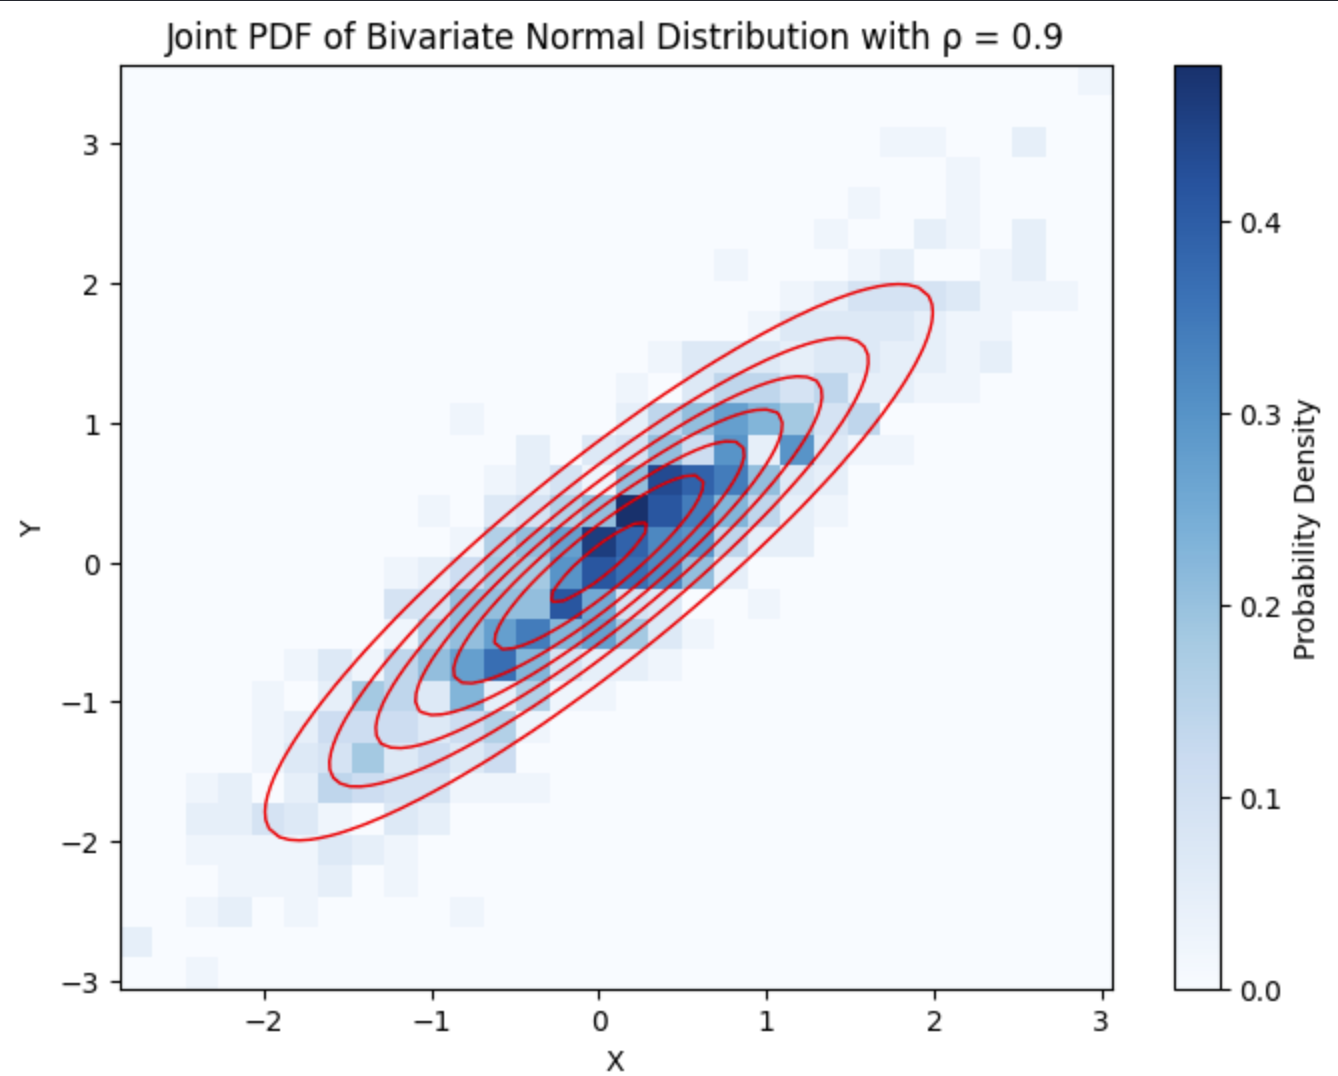
\includegraphics[width=0.23\textwidth]{0.9.png}
    \caption{Bivariate Normal Distributions with Different $\rho$ Values}
    \label{fig:bivariate_normal}
  \end{figure}
 
  

\end{homeworkProblem}







\begin{homeworkProblem}[3]
    \begin{enumerate}[(a)]
    \item 
    According to the memoryless property of exponential distribution, we have $E(X - 2024|X > 2024) = E(X)$. We can obtain the conditional expectation as follows:
    \[
        E(X|X > 2024) = 2024 + E(X - 2024|X > 2024) = 2024 + E(X) = 2023 + \frac{1}{\lambda_1}
    \]

    \item 
    According to the formula of LOTUS:
    \[
        E(X|X < 1997) = \int_{0}^{1997} x \cdot f_{X|A}(x) \, dx = E(X_1 | X_1 < 1997) = \int_{0}^{1997} x \cdot \frac{\lambda e^{-\lambda x}}{1 - e^{-1997\lambda}} \, dx
    \]
    \[
        E(X|X < 1997) = -(1997\lambda + 1)e^{-1997\lambda} + 1
    \]
    \item 
    We know that $X_1$, $X_2$, $X_3$ are independent, so we have:\\
    \begin{align*}
        E(X_1 + X_2 + X_3&|X_1 > 1997, X_2 > 2014, X_3 > 2025) = E(X_1|X_1 > 1997, X_2 > 2014, X_3 > 2025)\\
        &+ E(X_2|X_1 > 1997, X_2 > 2014, X_3 > 2025) + E(X_3|X_1 > 1997, X_2 > 2014, X_3 > 2025)\\
        &= E(X_1|X_1 > 1997) + E(X_2|X_2 > 2014) + E(X_3|X_3 > 2025)\\
        &= E(X_1 - 1997|X_1 > 1997) + E(X_2 - 2014|X_2 > 2014) + E(X_3 - 2025|X_3 > 2025) + 6036\\
        &= E(X_1) + E(X_2) + E(X_3) + 6036\\
        &= \frac{1}{\lambda_1} +  \frac{1}{\lambda_2} +  \frac{1}{\lambda_3} + 6036
    \end{align*}

    \end{enumerate}
\end{homeworkProblem}


\begin{homeworkProblem}[4]

\end{homeworkProblem}


\begin{homeworkProblem}[5]

\end{homeworkProblem}


\begin{homeworkProblem}[6]

\end{homeworkProblem}


\end{document}
